
\documentclass[12pt, a4paper]{article}

\usepackage[utf8]{inputenc}
\usepackage[T1]{fontenc}
\usepackage[russian]{babel}
\usepackage[oglav,spisok,boldsect,eqwhole,figwhole,hyperref,hyperprint,remarks,greekit]{./style/fn2kursstyle}
\graphicspath{{./style/}{./figures/}}

\usepackage{multirow}
\usepackage{supertabular}
\usepackage{multicol}
\usepackage{amsmath}
\usepackage{afterpage}
\usepackage{graphicx}
% Параметры титульного листа
\title{Вариант 8}
\author{В.\,Г.~Пиневич}
\supervisor{И.\,Ю.~Савельева}
\group{ФН2-81Б}
\date{2024}

% Переопределение команды \vec, чтобы векторы печатались полужирным курсивом
\renewcommand{\vec}[1]{\text{\mathversion{bold}${#1}$}}%{\bi{#1}}
\newcommand\thh[1]{\text{\mathversion{bold}${#1}$}}
%Переопределение команды нумерации перечней: точки заменяются на скобки
\renewcommand{\labelenumi}{\theenumi)}
\begin{document}

\maketitle

\tableofcontents



\newpage

\section{Постановка задачи}
Провести расчет изменения параметров газообразных продуктов сгорания топ-
лива при их адиабатическом истечении через сопло ракетного двигателя. Продукты
сгорания соответствуют модели совершенно невязкого(идеального) газа. Вычислить
площади $F_*$, $F_3$ и диаметры $D^*$, $D_3$ критического и выходного сечений сопла соответ-
ственно. Используя формулу Вентцеля, вычислить скорость $\omega$ истечения газа
из сопла и затем по следующей из закона сохранения импульса(количества движения) формуле $P = \dot{m} \omega + \left(p_3 - p_0\right)F_3$, где $p_0$ --- давление окружающей среды, рассчитать
силу $P$ тяги двигателя при его работе на Земле и в пустоте. Построить графики зависимостей давления $p$, температуры $T$, плотности $r$ и скорости $u$ газового потока от относительной площади $\overline{F} = F / F_* \in [1, F_3 / F_*]$ поперечного сечения сверхзвуковой
части сопла.

\section{Решение}
Рассмотрим адиабатический процесс движения газа. Объемные источники тепловыделения отсутствуют, следовательно процесс изоэнтропический. Так как процесс
адиабатический, справедливо следующее выражение:
\begin{equation}
	\label{first}
\frac{T}{p^{\kappa - 1}} = \frac{T_1}{p^{\kappa - 1}_1}, \kappa = \frac{c_p}{c_u}
\end{equation}

Из уравнения состояния совершенного газа
\[
p = \rho R_g T
\]
\noindent получим выражения для плотности газа в камере сгорания 
\[
\rho_1 = \frac{p_1}{R_g T_1}
\]
из соотношения~(\ref{first}) следует, что
\[
\frac{T_3}{T_1} = \frac{\rho_3}{\rho_1}^{\kappa - 1} = \frac{p_3}{p_1}^{\frac{\kappa - 1}{\kappa}}
\]
выразим и найдем плотность газа в выходном сечении
\[
\rho_3 = \rho_1 \left(\frac{p_3}{p_1}\right)^{\frac{1}{\kappa}}
\]

Найдем площадь критического состояния из соотношения
\[
\frac{\dot{m}}{F_*} = \sqrt{\frac{2 \kappa R_g T_1^*}{\kappa - 1} \rho_3^2 \left(1 - {\left(\frac{p_3}{p_1}\right)}^{\frac{\kappa - 1}{\kappa}} \right)}
\]

Найдем площадь критического сечения из соотношения
\[
\frac{\dot{m}}{F_*} = \left(\frac{2}{\kappa + 1}\right)^{\frac{\kappa + 1}{2 \left(\kappa - 1\right)}} \sqrt{\kappa \rho_1 p_1}
\]
С помощью формулы Вентцеля вычислим скорость $\omega$ истечения газа из сопла
\[
u = \sqrt{\frac{2 \kappa R_g T_1^*}{\kappa - 1}} \left(1 - \left(\frac{p}{p_1}\right)^{\frac{\kappa - 1}{\kappa}} \right)
\]
По формуле, следующей из закона сохранения импульса
\[
P = \dot{m} \omega + \left(p_3 - p_0\right) F_3
\]
Рассчитаем силу $P$ тяги двигателя при его работе на Земле ($P_e$) и в пустоте($P_0$). Атмосферное давление на Земле $p_e$ будем считать равным 1 атмосфере ($10^5$ Па). При работе двигателя в пустоте давление снаружи равно нулю. Таким образом, выражеsния для силы тяги примут вид
\[
P_e = \dot{m} \omega + \left(p_3 - p_e\right) F_3
P_0 = \dot{m} \omega + p_3 F_3
\]
Определим характеристики газа в критическом сечении
\[
\frac{p_*}{p_1} = \frac{2}{\kappa + 1}^{\frac{\kappa}{\kappa + 1}}
\]
Из закона сохранения массы
\[
\frac{\dot{m}}{F_*} = \rho_* u_* \rightarrow u_* = \frac{\dot{m}}{\rho_* F_*}
\]
Результаты вычислений:
\[
\begin{cases}
	F_* = 0.033,\\
	F_3 = 1.19,\\
	D_* = 0.21,\\
	D_3 = 1.23,\\
	\omega = 3701.83,\\
	P_e = 1.17 \cdot 10^6,\\
	P_0 = 1.29 \cdot 10^6
\end{cases}
\]


	\begin{figure}[!htbp]
		\centering
		\begin{minipage}[b]{0.4\textwidth}
		{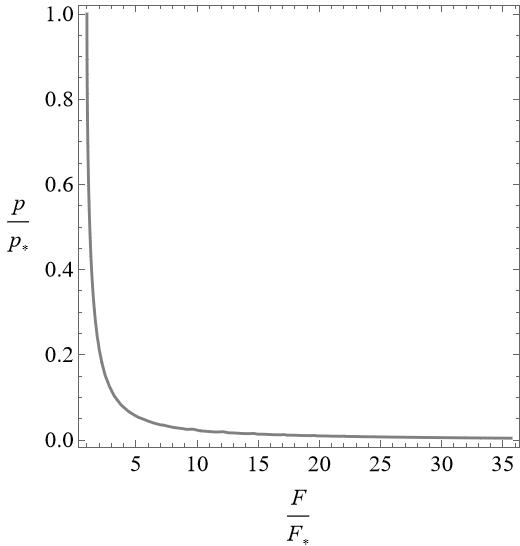
\includegraphics[width=\textwidth, height=\textwidth]{plot1}}
		\caption{Зависимость $P$ от $\overline{F}$}
		\end{minipage}
		\hfill
		\begin{minipage}[b]{0.4\textwidth}
		{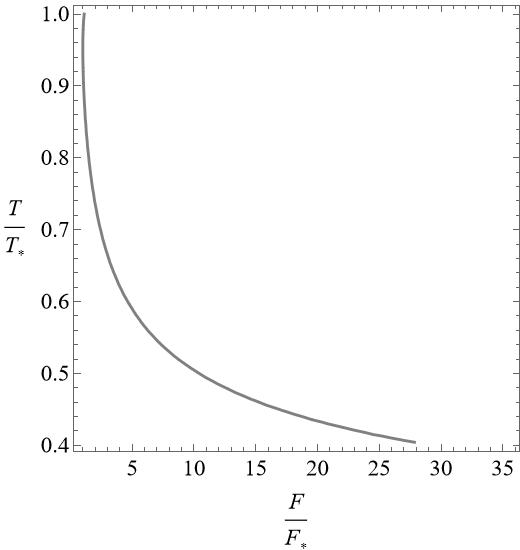
\includegraphics[width=\textwidth, height=\textwidth]{plot2}}
		\caption{Зависимость $T$ от $\overline{F}$}
		\end{minipage}
		\label{plot-1-2}
	\end{figure}

	\begin{figure}[!htbp]
		\centering
		\begin{minipage}[b]{0.4\textwidth}
			{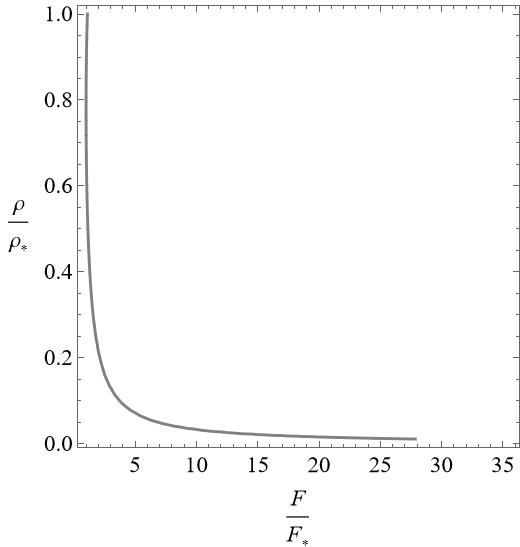
\includegraphics[width=\textwidth, height=\textwidth]{plot3}}
			\caption{Зависимость $\rho$ от $\overline{F}$}
		\end{minipage}
		\hfill
		\begin{minipage}[b]{0.4\textwidth}
			{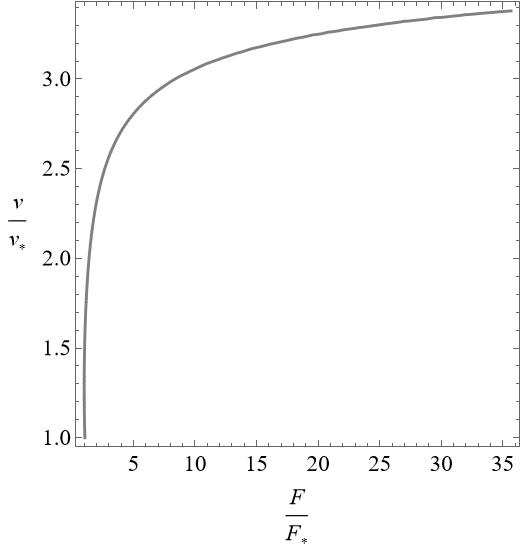
\includegraphics[width=\textwidth, height=\textwidth]{plot4}}
			\caption{Зависимость $u$ от $\overline{F}$}
		\end{minipage}
		\label{plot-3-4}
	\end{figure}



\end{document} 